Since the beginning of time, humans were eager to explore their environment and surroundings. It did not take long, until the first humans started getting even further and become explorers. They started leaving marks and using landmarks to remember pathways and places. This primitive representation of prehistoric places and early history maps can be traced back to 24000-25000 BC. Soon after, they started using maps which revolutionized the way we navigate and the way we travel, and therefore the field of Cartography become a reality. During the 19th century terra incognita disappeared from maps, since both the coastlines and the inner parts of the continents had been fully explored. Today, using technology and satellites, Earth is completely mapped, yet still not completely explored. Around 95 percent of our oceans are still remain unexplored, considering that they take up 70 percent of the planet's surface. This is mostly due to extreme conditions and high depths, that humans can not be put up against. Remotely operated underwater vehicles (ROVs) become a popular way of exploring the depths of our oceans and they are still being developed by many around the world. In the meantime, interplanetary exploration took off during the mid-20th century with the start of the Cold War between the United States of America and the Soviet Union. This led to many great achievements, like the first successful interplanetary encounter, where the US Mariner 2 fly by Venus or when the Soviet Venera 3 made first impact on the surface of Venus.


\begin{figure}[!htb]
	\centering
	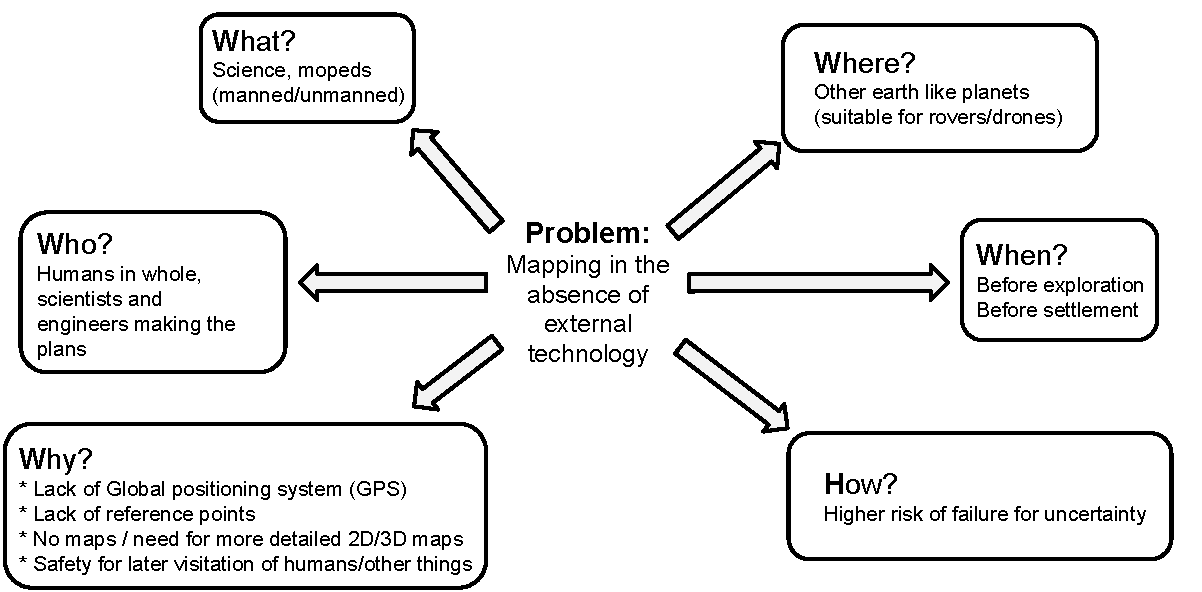
\includegraphics[scale=.7]{images/wdiagram1.pdf}
	\caption{W-diagram}
	\label{fig:wdiagram}
\end{figure}

%http://wwws.phil.uni-passau.de/histhw/tutcarto/english/index-frames-en.html
%http://www.e-perimetron.org/Vol_2_2/Wolodchenko_Forner.pdf
%http://en.wikipedia.org/wiki/Terra_incognita
%http://en.wikipedia.org/wiki/History_of_cartography
%http://oceanservice.noaa.gov/facts/exploration.html